\chapter{Optimization}

\section{Overview}
    As we have detailed earlier, we will conclude this thesis with the optimization of some of the parameters we have seen and analyzed, namely the 4 taxes (VAT, Levy, Tariff and Wealth tax), the unemployment rate and the black economy share in order to improve different metrics which will be used as the objective function, namely the Gini coefficient (to be minimized), the GDP (to be maximized) and the number of transactions (to be maximized). We will focus on a single objective (for instance the Gini coefficient) at the time while optimizing a solution with 6 dimensions (4 taxes + 2 rates) stored in a list as follows: \texttt{[VAT, LEVY, TARIFF, WEALTH\_TAX, UNEMPLOYMENT, BLACK\_ECONOMY]}(which represents the DNA in the Genetic Algorithm or a particle in the PSO). All values are, of course, in the range $[0, 1]$. For the optimization, we use another default configuration file \texttt{templateOptimization.json} with only one State, 1000 agents and 2000 ticks.
    
    As mentioned in the section~\ref{section:state_of_the_art} \nameref{section:state_of_the_art}, we will use population-based methods as they allow us multiple configurations (Worlds with different parameters) in parallel: the genetic algorithm (GA) and particle swarm optimization (PSO).

\section{Algorithms}

    \subsection{Genetic Algorithm}

    The first optimization algorithm which was tried is the genetic algorithm (GA) as explained in the state-of-the-art. The algorithm was developed from scratch and it used the following operators:

        \paragraph{Initialization} A population of candidate solutions is generated at random. Each candidate solutions has its own DNA: \texttt{[VAT, LEVY, TARIFF, WEALTH\_TAX, UNEMPLOYMENT, BLACK\_ECONOMY]}.

        \paragraph{Selection} The 20\% best of the population (with the highest fitness) were kept to undergo reproduction (crossover).

        \paragraph{Crossover} Two crossover were tested: the uniform and the 1 point crossover. The uniform crossover will, for each solution component, either copy it from parent 1 or from parent 2 according to a certain probability. The 1 point crossover will choose one point in the DNA. All solution components before that point will be copied from the first parent, and all solution components after that point will be copied into the offspring from the second parent.

        \paragraph{Mutation} According to a certain mutation rate, we will stochastically mutate one solution component in the candidate solution. The replacing solution component is taken at random in $[0, 1]$.

        \paragraph{Results} Unfortunately, this GA resulted in quite poor results, no clear pattern was emerging. The main hypothesis of why such a behavior happened is that the crossover operations were not fitted for such a problem where the different solution components are very independent from one another, and cannot simply be copied partially. The algorithm has been deleted (but remains available in a previous commit on the Github repository)

    \subsection{Particle Swarm Optimization}

    The first optimization algorithm which was tried is the Particle swarm optimization (PSO) as explained in the state-of-the-art. This time, instead of redoing everything from scratch, a python3 library was used: \texttt{pyswarms}. We used a swarm of 50 particles for 50 iterations with $\phi_1 = 0.5$ and $\phi_2 = 0.3$ (therefore advantaging exploration/diversification). We also set the inertia parameter $w$ to $0.9$. This parameter is used to control the particles' speed of convergence, we favour, again, diversification of the search process by setting it this high. \cite{psoDorigo} Other hyper-parameters have been tested (such as a very low inertia, and a $\phi_1$ smaller than $\phi_2$ to favor intensification instead), however, due to the high number of particles and iterations, no significant improvements have been noticed.
    
    This algorithm has proven itself to be much better than the GA, hence we will analyze the solutions is has computed. 

\section{Analysis}
    Whenever we try one configuration, we run it 3 times, and average the resulting fitnesses in order to take into account the stochasticity of the simulation. We will analyze three optimized metrics: the Gini coefficient (to be minimized), the GDP (to be maximized) and the number of transactions (to be maximized). For each of them, we will run the optimization algorithm 10 times in order to see the results produced. We do 10 times in order to see the optimized parameters that were found, and see if, there are any patterns between the 10 solutions found. It takes around 19 hours on the cluster for everything to run (3 metrics * 10 PSOs made of 50 iterations of 50 particles with 3 simulations averaged).

    \subsection{Gini coefficient}

        Usually, we want to decrease the inequalities between the agents of a State, therefore we should optimize the Gini coefficient by minimizing it. The following results were obtained.
    
        \subsubsection{Optimized parameters}
        \begin{table}[H]
        \centering
        \begin{tabular}{|c|c|c|c|c|c|c|c|}
            \hline
            \textbf{\#} & \textbf{Gini}  & \textbf{VAT} & \textbf{Levy} & \textbf{Tariff} & \textbf{Wealth} & \textbf{Unemployment} & \textbf{Black} \\ \hline
            \textbf{1} & 0.0 & 0.783 & 0.999 & 1.0 & 0.209 & 0.333 & 0.201 \\ \hline
            \textbf{2} & 0.0 & 0.301 & 0.999 & 0.371 & 0.682 & 0.377 & 0.59 \\ \hline
            \textbf{3} & 0.0 & 0.018 & 0.998 & 0.753 & 0.434 & 0.998 & 0.828 \\ \hline
            \textbf{4} & 0.0 & 0.323 & 0.998 & 0.255 & 0.101 & 0.999 & 0.063 \\ \hline
            \textbf{5} & 0.0 & 0.915 & 0.999 & 0.458 & 0.65 & 0.525 & 0.656 \\ \hline
            \textbf{6} & 0.0 & 0.978 & 0.999 & 0.808 & 0.946 & 0.022 & 0.533 \\ \hline
            \textbf{7} & 0.0 & 0.215 & 0.757 & 0.784 & 0.142 & 0.999 & 0.299 \\ \hline
            \textbf{8} & 0.0 & 0.618 & 0.999 & 0.334 & 0.658 & 0.657 & 0.633 \\ \hline
            \textbf{9} & 0.0 & 0.437 & 1.0 & 0.731 & 0.965 & 0.836 & 0.532 \\ \hline
            \textbf{10} & 0.0 & 0.538 & 0.999 & 0.763 & 0.554 & 0.445 & 0.461 \\ \hline
        \end{tabular}
        \end{table}

        We see that all optimization runs could lower the Gini coefficient to 0, i.e. perfect equality. We can see that the Levy tax is the one who is almost at the same for all the optimizations, i.e. it is the most important parameter influencing the Gini coefficient.  This makes sense, because as detailed in \nameref{exp:levy}, if we levy close to 100\% of the money of all agents, and then redistribute, they will all get the same money therefore greatly reducing inequalities. However, this result can, of course, difficulty be applied in real life. 
        
        We can also see that one optimization has not reach a very high VAT of $\approx 0.999$ which is the \#7, this is quite peculiar but it is explained by the high level of unemployment of $0.999$. If all agents do not produce, naturally they will be as poor, therefore receive the same (very small) allowance making them quite equal.

        We can also see in the following plot the decrease of the Gini coefficient across iterations (cost history):

        \begin{figure}[H]
            \centering
            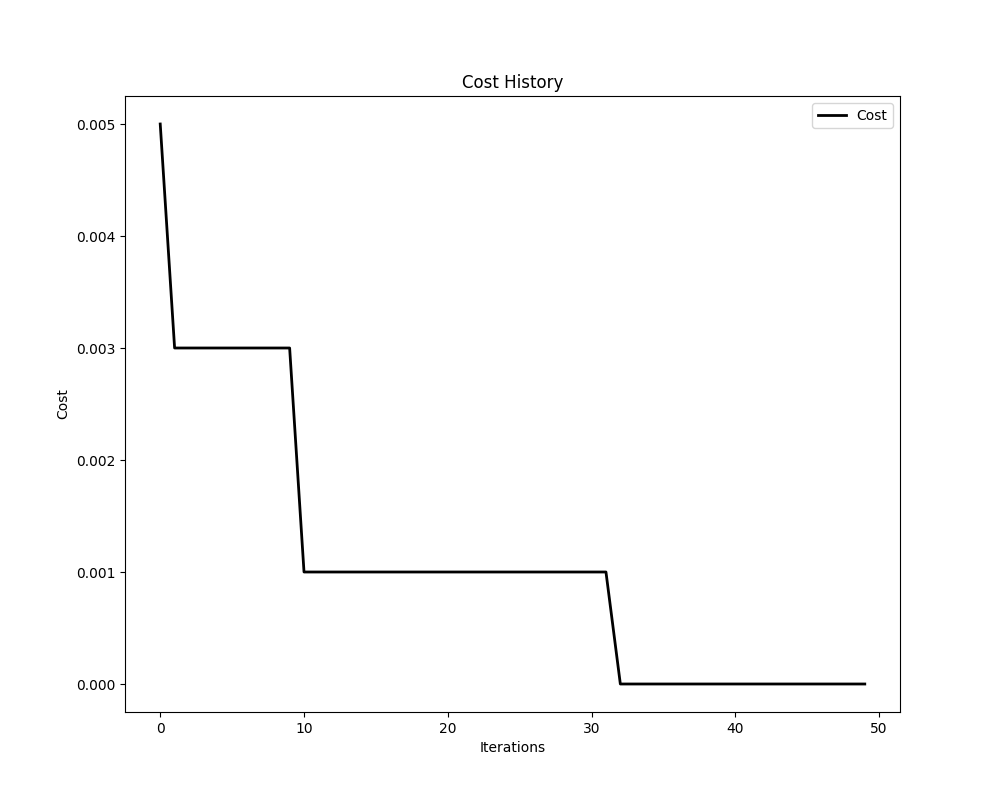
\includegraphics[width=0.9\textwidth]{img/opti/costHistoryGini.png}
            \caption{Cost history of the Gini coefficient}
        \end{figure}

        \subsubsection{Statistical analysis}
        %TODO
        

    \subsection{GDP}

        Naturally, we want to maximize the GDP of a State. The following results were obtained.
    
        \subsubsection{Optimized parameters}
        \begin{table}[H]
        \centering
        \begin{tabular}{|c|c|c|c|c|c|c|c|}
            \hline
            \textbf{\#} & \textbf{GDP}  & \textbf{VAT} & \textbf{Levy} & \textbf{Tariff} & \textbf{Wealth} & \textbf{Unemployment} & \textbf{Black} \\ \hline
            \textbf{1} & 36 739 & 0.043 & 0.729 & 0.376 & 0.769 & 0.309 & 0.036 \\ \hline
            \textbf{2} & 37 152 & 0.054 & 0.651 & 0.272 & 0.988 & 0.175 & 0.018 \\ \hline
            \textbf{3} & 36 749 & 0.059 & 0.945 & 0.528 & 0.021 & 0.337 & 0.034 \\ \hline
            \textbf{4} & 37 691 & 0.005 & 0.994 & 0.675 & 0.66 & 0.268 & 0.052 \\ \hline
            \textbf{5} & 36 334 & 0.0 & 0.846 & 0.537 & 0.833 & 0.387 & 0.014 \\ \hline
            \textbf{6} & 36 453 & 0.001 & 0.819 & 0.443 & 0.209 & 0.077 & 0.081 \\ \hline
            \textbf{7} & 36 703 & 0.043 & 0.91 & 0.505 & 0.285 & 0.13 & 0.006 \\ \hline
            \textbf{8} & 35 130 & 0.025 & 0.47 & 0.525 & 0.51 & 0.285 & 0.082 \\ \hline
            \textbf{9} & 35 556 & 0.198 & 0.944 & 0.37 & 0.957 & 0.423 & 0.028 \\ \hline
            \textbf{10} & 36 339 & 0.109 & 0.924 & 0.519 & 0.426 & 0.096 & 0.047 \\ \hline
        \end{tabular}
        \end{table}

        We can see some interesting patterns in the table. Indeed, we see that the VAT rates are very close to one another, the same goes for the black economy share. This actually fits our state-of-the-art and our experiments. Indeed, if we see, for instance, in \nameref{exp:black}, we had noticed that, as the black economy share grows, the GDP decreases. Therefore, reducing black economy at such low levels drastically increases the GDP.
        On the other side, we see no real pattern for the other parameters, i.e. they do not significantly influence the GDP.

        We can also see in the following plot the decrease of the GDP across iterations (cost history). PSO will minimize the opposite of the GDP (thus maximizing the GDP), that is why the costs are negative, and we want them to be as low as possible.

        \begin{figure}[H]
            \centering
            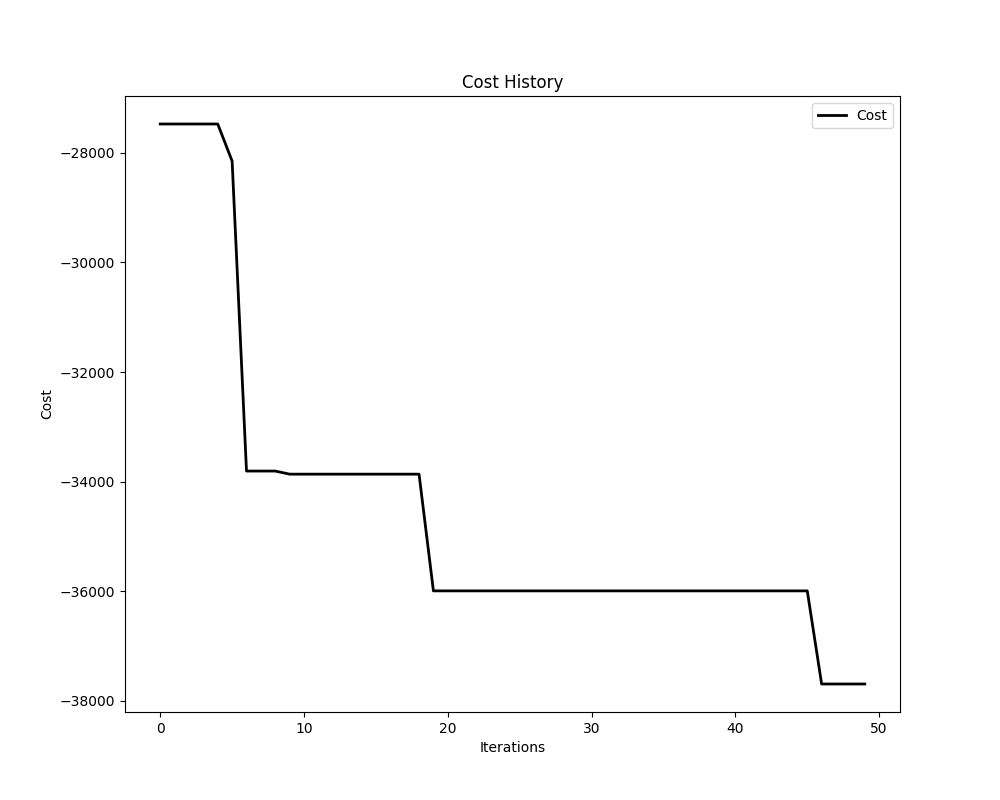
\includegraphics[width=0.9\textwidth]{img/opti/costHistoryGDP.png}
            \caption{Cost history of the GDP}
        \end{figure}

        \subsubsection{Statistical analysis}
        %TODO

    \subsection{Number of transactions}

        Naturally, we want to maximize the number of transactions in a State. The following results were obtained.
    
        \subsubsection{Optimized parameters}
        \begin{table}[H]
        \centering
        \begin{tabular}{|c|c|c|c|c|c|c|c|}
            \hline
            \textbf{\#} & \textbf{Nb transactions}  & \textbf{VAT} & \textbf{Levy} & \textbf{Tariff} & \textbf{Wealth} & \textbf{Unemployment} & \textbf{Black} \\ \hline
            \textbf{1} & 739 & 0.456 & 0.824 & 0.487 & 0.556 & 0.021 & 0.954 \\ \hline
            \textbf{2} & 788 & 0.741 & 0.871 & 0.18 & 0.462 & 0.063 & 0.996 \\ \hline
            \textbf{3} & 753 & 0.708 & 0.906 & 0.939 & 0.884 & 0.041 & 0.993 \\ \hline
            \textbf{4} & 737 & 0.419 & 0.691 & 0.137 & 0.551 & 0.005 & 0.826 \\ \hline
            \textbf{5} & 726 & 0.091 & 0.924 & 0.904 & 0.175 & 0.044 & 0.714 \\ \hline
            \textbf{6} & 752 & 0.412 & 0.759 & 0.554 & 0.671 & 0.004 & 0.917 \\ \hline
            \textbf{7} & 747 & 0.608 & 0.974 & 0.588 & 0.743 & 0.005 & 0.957 \\ \hline
            \textbf{8} & 725 & 0.306 & 0.682 & 0.55 & 0.794 & 0.062 & 0.962 \\ \hline
            \textbf{9} & 740 & 0.963 & 0.858 & 0.323 & 0.472 & 0.018 & 0.994 \\ \hline
            \textbf{10} & 746 & 0.672 & 0.479 & 0.073 & 0.809 & 0.001 & 0.954 \\ \hline
        \end{tabular}
        \end{table}

        We can see two patterns emerging. First, for the number of transactions to be high, we need a very small unemployment rate as we can see on the table (i.e. this is the `common denominator' of all these optimizations). This makes sense, because more unemployment means more non-producers, therefore less products on the market to buy and less transactions. This fits our \nameref{exp:unemployment} where we saw a linear correlation between the unemployment rate and the number of transactions.

        Secondly, we can see that, generally but not always, the black economy share is very high. This is due to the fact that a black transaction is still counted towards the total number of transactions, however no due taxes are paid. This is quite surprising as it is not exactly what we had seen in \nameref{exp:black} where we saw no real correlation between the black economy share and the number of transactions.

        We can also see in the following plot the decrease of the number of transactions across iterations (cost history). PSO will minimize the opposite of the number of transactions (thus maximizing the number of transactions), that is why the costs are negative, and we want them to be as low as possible.

        \begin{figure}[H]
            \centering
            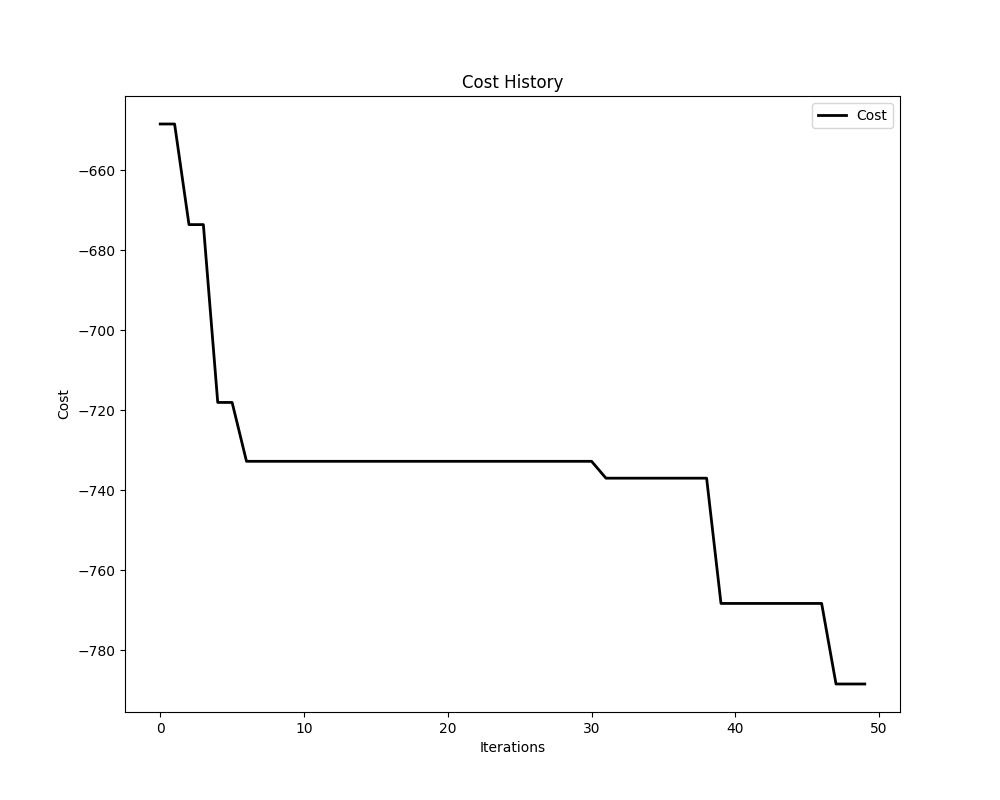
\includegraphics[width=0.9\textwidth]{img/opti/costHistoryNbTransactions.png}
            \caption{Cost history of the number of transactions}
        \end{figure}


        \subsubsection{Statistical analysis}
        %TODO

